\begin{abstract} Faceted search has been recognized as an eminent tool for
assisting users in discovering relevant topics in digital library applications.
Conventional count-based presentation scheme usually presents the discovered
facets according to the corresponding numbers of counts in the result set,
without considering the relevance between the facet and the query.  We argue
that this approach might work well only when the retrieved documents are all
highly relevant, which is not usually the case in the real-world query
sessions.  In this work,  we investigated an alternative solution for ranking
the discovered facets.  We proposed a generative Bayesian framework to better
account for different degrees of the relevant contribution from the retrieved
documents to the discovered facets.  The evaluation result showed that our
method significantly outperformed the baseline approach, improving the
retrieval accuracy from 33\% to 100\% in terms of mean-average precision.
\end{abstract}

\section{Introduction}

In the past few years, faceted search has gained wide acceptance in the digital
library and the Web community.  We have seen many successful applications of
this search technique in different domains, including the Web
\cite{hearst2002finding}, image collections \cite{yee2003faceted}, and database
catalogs \cite{roy2008minimum}; the technique has also given rise to a number
of interesting research results that application developers could immediately
benefit from, such as the usability of the faceted interface
\cite{kules2009what} and the approach for automatically extracting facets from
the texts \cite{mimno2007organizing}.  

Generally, faceted search can be seen as a two-phase extension of the ordinary
retrieval task: In the first phase, one populates a set of document
(\emph{result set}) by querying the underlying retrieval model; then, in the
second phase, one exploits the associations between the facet entries and the
documents, and returns the facet items back to the users.  In mathematical
terms, supposed that the result set of query $\mathbf{q}$ is denoted as $R_{q}$
and the associated facet items of document $d$ is represented as a set $F_d$,
we expect the faceted interface returns this set of facet items: \[ \{ f \in
F_d | d \in R_{\mathbf{q}} \}.  \] Conventionally, these discovered facets are
presented in descending order of the number of corresponding occurrences in the
result set, which we called ``count-based'' scheme.  \footnote{In very few
cases that we has noted, the facets are presented in lexicographical order.}
The count-based scheme has a number of advantages, including its being fast,
being easy to implement, and being simple and straightforward in the user
interface design.  However, with this style of presentation the users is
unaware of the the \emph{relevance} of the discovered facets to the query.  The
incapability to address relevance might sometimes result in bitter user
experience.  In one hand, if we assume that all the documents that match the
query topic are equally relevant, then the ranking of the facets might not be
so important.  On the other hand, on the systems that equipped with
fuzzy-matching search facilities, documents at different ranks pose different
degrees of relevance; therefore, the facets triggered by documents at different
ranks should be accounted for differently.  In real-world applications, we find
the latter case occurs more often than the former.  We define the task for
assigning appropriate importance or relevance to facet as \emph{facet ranking}.

Our work serves as a preliminary study toward good facet ranking algorithms,
largely motivated by the impression that improvements on facet ranking leads to
better user experience for faceted search in digital library systems.  In this
paper, we propose an alternative solution to take the place of the count-based
method by ranking the discovered facet based their relevance to the query.  We
conducted a series of experiments on a custom benchmark, and show that our
proposed method outperforms the regular count-based approach in regular query
sessions, achieving high improvement in terms of mean-average precision and
precision-at-10.

The rest of the work is organized as follows: We introduce a Bayesian language
modeling approach in Section~\ref{s:model} and propose two different models for
facet ranking.  We further elaborate the proposed solutions in
Section~\ref{s:inference}.  Section~\ref{s:experimental-setup} presents the
experiment for evaluating the proposed methods, and the creation of the
benchmark; the experimental result is shown in Section~\ref{s:results}.  We
briefly summarize the related work in Section~\ref{s:related-work}; finally, we
discuss a few issues raised in the development of the work and give out
concluding remarks in Section~\ref{s:concluding-remarks}.

\section{Model}\label{s:model}

An intuitive way to induce a ranking mechanism is by considering the relevance
scores contributed by the documents that covers the target facet.  For example,
the facet covered by a highly-relevant document should be assigned a higher
weight, and the facet found in documents that get low relevance scores should
be ranked lower accordingly.  Since different documents might contribute
different degrees of relevance to the facet and each such facet being
considered here is at least covered by one or more documents from the result
set, a weighted-sum model may serve the purpose well.  Based on this idea, our
goal is to model the contribution of relevance from a document to a facet by
exploiting the underlying retrieval model.  Besides, we find it more appealing
to apply this technique on a language-model-based backend, since the document
relevance score can be easily integrated into the final ranking results; the
detail is elaborated in Section~\ref{ss:integration}.

First, we model the task as a Bayesian generative process.  Let $D$ denotes the
document domain, $T$ the term domain, and $F$ the facet domain.  Consider a
document collection of size $N$, in which each document $d_j$ is associated
with a set of terms $T_j$ and a set of facets $F_j$.  We assume that each term
$t_i \in T_j$ and each facet $f_k \in F_j$ are drawn from from two
document-specific multinomials embedded in document $j$, one over the term
domain and the other over the facet domain, respectively.  We further assume
that the former distribution, denoted as $\tau^{(j)}$, is drawn from a
Dirichlet prior $\{ \alpha_i; i \in [1, T] \}$ and the latter from another
Dirichlet $\{ \beta_k; k \in [1, F] \}$.  The generative process can be
described as follows: \footnote{A formal way to model the generation of the
corresponding set size $|T_j|$ and $|F_j|$ is through Poisson processes.  For
simplicity, in this work we assume these numbers are pre-determined for each
document $d_j$.} 

\begin{itemize} 
  \item For each document $d_j$, \begin{enumerate}
    \item $\tau^{(j)} \sim \textrm{Dirichlet}(\alpha_i; i \in [1, |T|])$
    \item $\phi^{(j)} \sim \textrm{Dirichlet}(\beta_k; i \in [1, |F|])$
    \item For $i \in \{ 1, \ldots, |T_j| \}$, $t_i \sim \textrm{Mult}(\tau^{(j)})$ 
    \item For $k \in \{ 1, \ldots, |F_j| \}$, $f_k \sim \textrm{Mult}(\phi^{(j)})$ 
  \end{enumerate}
\end{itemize}

Then, we consider the input query $\mathbf{q}$ as a new document $x$ in the
framework, in which a set of observable variables associated with $x$ are the
query terms $q_i$'s.  The value $x$ is currently unknown, and it is associated
with another unknown variable $y$ represent the most-likely facet generated by
$x$.  Since our goal is to rank facets, one facet node that represents the most
probable one is as good as many.  The idea behind such an arrangement is that
we wish to explicitly model the likelihood of a facet being triggered in the
model.  That is, through the search for the most likely document model $x$
behind the query terms, we may also get good probabilistic estimate on the
likelihood for triggering $y$.

Now, in this framework there are two obvious solutions to rank the facets.  In
the first case, which we coin as the \emph{forward model}, we search for the
most probable facet $f$ triggered by the query $\mathbf{q}$:
\begin{equation}y^*_{\rm f} = \arg\max_{y \in F} \Pr(y|\mathbf{q}, \mathbf{t},
\mathbf{d}, \mathbf{f}) \label{eq:forward} \end{equation} In the second case,
the search is done in \emph{backward} by looking for the most probable facet
$f$ that triggers the query $\mathbf{q}$:  \begin{equation}y^*_{\rm b} =
\arg\max_{y \in F} \Pr(\mathbf{q}|y, \mathbf{t}, \mathbf{d}, \mathbf{f}).
\label{eq:backward} \end{equation} 

Here, we coin the term \emph{trigger} because there is no direct
ancestor/descendant relation between the facet nodes and the term nodes.  The
full generative process is shown in Figure~\ref{f:model}.  

\begin{figure}[ht!]
  \centering
  \psset{xunit=10mm,yunit=10mm}
  \begin{pspicture}(0,-2)(8,5)%\showgrid  % Uncomment to show grid!
    \SpecialCoor  % (a|b) means x-coord from 'a' and y-coord from 'b'.
    \psset{arrowscale=1.5}
    \rput(4.0,0.0){\GM@node[observed=true]{d}}\GM@label[angle=90]{d}{$d_j = j$}
    \rput(2.0,0.0){\GM@node[observed=true]{t}}\GM@label[angle=45]{t}{$t_i$}
    \rput(1.25, -0.75){\GM@plate{1.5}{1.5}{$|T_j|$}}
    \rput(6.0,0.0){\GM@node[observed=true]{f}}\GM@label[angle=45]{f}{$f_k$}
    \rput(5.25, -0.75){\GM@plate{1.5}{1.5}{$|F_j|$}}
    \rput(0.75, -1.25){\GM@plate{6.5}{2.5}{$N$}}

    \rput(4.0,4.0){\GM@node{x}}\GM@label[angle=45]{x}{$x$}
    \rput(2.0,4.0){\GM@node[observed=true]{q}}\GM@label[angle=45]{q}{$q_i$}
    \rput(1.25, 3.25){\GM@plate{1.5}{1.5}{$|Q|$}}
    \rput(6.0,4.0){\GM@node{y}}\GM@label[angle=45]{y}{$y$}

    \rput(2.0,2.0){\GM@node{tau}}\GM@label[angle=45]{tau}{$\tau$}
    \rput(6.0,2.0){\GM@node{phi}}\GM@label[angle=45]{phi}{$\phi$}
    \rput(0.0,0|tau){\GM@parameter{alpha}}\GM@label[angle=45]{alpha}{$\alpha$}
    \rput(8.0,0|phi){\GM@parameter{beta}}\GM@label[angle=45]{beta}{$\beta$}

    \ncline[arrows=->]{d}{t}
    \ncline[arrows=->]{d}{f}
    \ncline[arrows=->]{x}{q}
    \ncline[arrows=->]{x}{y}
    \ncline[arrows=->]{tau}{t}
    \ncline[arrows=->]{tau}{q}
    \ncline[arrows=->]{phi}{f}
    \ncline[arrows=->]{phi}{y}
    \ncline[arrows=->]{alpha}{tau}
    \ncline[arrows=->]{beta}{phi}
  \end{pspicture}

  \caption{A document-centric generative model in the plate notation.  The
  document $d_j$ generates a set of terms $T_j$ in which each term is
  represented as $t_i$; meanwhile, the document is associated with a set of
  facets $F_j$ in which each facet is denoted as $f_k$.  The query terms are
  represented as $q_i$'s, which are generated from an unknown document model
  $x$; the document is associated with an unknown facet $y$.  The core idea
  behind this framework is to induce the probability associated with $x$ and
  $y$.} \label{f:model}
\end{figure}

%--------------------------------------------------
% In the following section, we show that both the forward and the backward models
% differ only slightly on how the score is normalized.  In the backward model,
% the facet score is normalized over the summation of the facet prior, which
% addresses the likelihood for a facet being generated; this step is unneccessary
% in the forward model.  
%-------------------------------------------------- 

\section{Inference}\label{s:inference}

\subsection{The Forward Model}\label{ss:forward-model}

We begin by deriving the solution for the forward model shown in
Equation~\eqref{eq:forward}. 
\begin{eqnarray}
  \Pr(y|\mathbf{q}, \mathbf{t}, \mathbf{d}, \mathbf{f}) 
  &=& \sum_{x \in [1, N]} \Pr(y|x, \mathbf{q}, \mathbf{t}, \mathbf{d}, \mathbf{f}) \Pr(x|\mathbf{q}, \mathbf{t}, \mathbf{d}, \mathbf{f}) \nonumber\\
  &\propto& \sum_{x \in [1, N]} \left\{ \int \Pr(y|x, \phi^{(x)}) \Pr(\phi^{(x)}|d_x, \mathbf{f_x}) \mathrm{d}\phi^{(x)} \right. \nonumber\\
  && \left. \int \Pr(\mathbf{q}| x, \tau^{(x)}) \Pr(\tau^{(x)}|d_x, \mathbf{t_x})\mathrm{d}\tau^{(x)} \Pr(x) \right\} \nonumber\\
  &=& \sum_{x \in [1, N]} \frac{\beta + c_{y,x}}{|F|\beta + c_{\cdot,x}} \frac{\mathcal{B}(\{\alpha_i + c_{i,x} + c_{i,q} \})}{\mathcal{B}(\{\alpha_i + c_{i,x} \})} \Pr(x) \label{eq:forward-solution}
\end{eqnarray}
Note that $\mathcal{B}(\cdot)$ is the multinomial beta
function defined by \[\mathcal{B}(a_1, \ldots, a_n) = \frac{\prod_i
\Gamma(a_i)}{\Gamma(\sum_i a_i)}. \]
The last line follows the conjugacy of Dirichlet distribution, as in:
\begin{eqnarray*}
\Pr(\phi^{(x)}|d_x,\mathbf{f_x}) &\sim& \mathrm{Dirichlet}(\{\beta_k + c_{k,x}; \forall k \}) \\
\Pr(\tau^{(x)}|d_x, \mathbf{t_x}) &\sim& \mathrm{Dirichlet}(\{\alpha_i + c_{i,x}; \forall i \}).
\end{eqnarray*}

\subsection{The Backward Model}\label{ss:backward-model}
The backward model shown in Equation~\eqref{eq:backward} is solved in similar way.
\begin{eqnarray}
  \Pr(\mathbf{q}|y, \mathbf{t}, \mathbf{d}, \mathbf{f}) 
  &=& \sum_{x \in [1, N]} \Pr(\mathbf{q}|x, y, \mathbf{t}, \mathbf{d}, \mathbf{f}) \Pr(x|y, \mathbf{t}, \mathbf{d}, \mathbf{f}) \nonumber\\
  &\propto& \sum_{x \in [1, N]} \left\{ \int \Pr(\mathbf{q}|x, \tau^{(x)}) \Pr(\tau^{(x)}|d_x, \mathbf{t_x}) \mathrm{d}\tau^{(x)} \right. \nonumber\\
  && \left. \int \Pr(y| x, \phi^{(x)}) \Pr(\phi^{(x)}|d_x, \mathbf{f_x})\mathrm{d}\phi^{(x)} \frac{\Pr(x)}{\Pr(y|\mathbf{t}, \mathbf{d}, \mathbf{f})} \right\} \nonumber\\
  &=& \frac{1}{\Pr(y|\mathbf{t}, \mathbf{d}, \mathbf{f})} \sum_{x \in [1, N]} \frac{\mathcal{B}(\{\alpha_i + c_{i,x} + c_{i,q} \})}{\mathcal{B}(\{\alpha_i + c_{i,x} \})} \frac{\beta + c_{y,x}}{|F|\beta + c_{\cdot,x}} \Pr(x) \nonumber
\end{eqnarray}

It is not difficult to see that the normalizing factor is in fact a similar summation.
$\Pr(y|\mathbf{t}, \mathbf{d}, \mathbf{f})$.
\begin{eqnarray}
  \Pr(y|\mathbf{t}, \mathbf{d}, \mathbf{f})
  &=& \sum_{x \in [1, N]} \Pr(y|x, \mathbf{t}, \mathbf{d}, \mathbf{f}) \Pr(x) \nonumber\\
  &=& \sum_{x \in [1, N]} \int \Pr(y|x, \phi^{(x)}) \Pr(\phi^{(x)}|d_x, \mathbf{f_x}) \mathrm{d}\phi^{(x)} \Pr(x) \nonumber\\
  &=& \sum_{x \in [1, N]} \frac{\beta + c_{y,x}}{|F|\beta + c_{\cdot,x}} \Pr(x) \nonumber
\end{eqnarray}

Therefore, the final form of Equation~\eqref{eq:backward} is as follow:
\begin{equation}\label{eq:backward-solution}
  \Pr(\mathbf{q}|y, \mathbf{t}, \mathbf{d}, \mathbf{f}) = 
  \frac{\sum_{x \in [1, N]} \frac{\mathcal{B}(\{\alpha_i + c_{i,x} + c_{i,q} \})}{\mathcal{B}(\{\alpha_i + c_{i,x} \})} \frac{\beta + c_{y,x}}{|F|\beta + c_{\cdot,x}} \Pr(x)}
  {\sum_{x \in [1, N]} \frac{\beta + c_{y,x}}{|F|\beta + c_{\cdot,x}} \Pr(x)}
\end{equation}

%--------------------------------------------------
% \begin{eqnarray}
%   \Pr(f|Q) &=& \sum_{d \in D} \Pr(f|d,Q) \Pr(d|Q) \nonumber\\
%   &=& \sum_{d \in D} \Pr(f|d) \Pr(d|Q) \nonumber\\
%   &\propto& \sum_{d \in D} \Pr(f|d) \Pr(Q|d) \label{eq:pr(f|Q)}\\
%   && \nonumber\\
%   \Pr(Q|d) &=& \prod_{q \in Q} \Pr(q|d) \nonumber\\
%   &\propto& \sum_{q \in Q} \log \Pr(q|d) \label{eq:pr(Q|d)}
% \end{eqnarray}
% 
% \paragraph{Estimation for $\Pr(Q|d)$.}
% 
% \begin{eqnarray}
%   \Pr(Q|d) &=& \exp \left(\sum_{q \in Q} \log \Pr(q|d) \right) \nonumber\\
%   &=& \exp \left(\sum_{q \in Q} \log \left[ \frac{f_{q,d} + \mu f_q / |C|}{|d| + \mu} \right] \right) \nonumber\\
%   &=& \exp \left(\sum_{q \in Q} \log \left( f_{q,d} + \mu f_q / |C| \right) - |Q| \log \left( |d| + \mu \right) \right) \nonumber\\
%   &=& K \times \exp \left( \sum_{q \in Q \cap d} \log \left( \frac{f_{q,d} |C|}{\mu f_q} + 1 \right) 
%   - |Q| \log \left( |d| + \mu \right) \right) 
% \end{eqnarray}
% where \[ K = \exp \left( |Q| \log \mu - |Q| \log |C| + \sum_{q \in Q} \log f_q \right). \]
% 
% \paragraph{Estimation for $\Pr(f|Q)$.}
% 
% \begin{eqnarray}
%   \Pr(f|Q) &\propto& \sum_{d \in D} \Pr(f|d) \Pr(Q|d) \nonumber\\
%   &=& \sum_{d \in \{d'|f \in d\}} \frac{c_{f,d}}{\mu_2 + c_d} \Pr(Q|d) + \sum_{d \in D} \frac{\mu_2 c_f / |F|}{\mu_2 + c_d} \Pr(Q|d)
% \end{eqnarray}
% 
% Let $c_{f,d} = 1$ and $K_f = \mu_2 c_f/|F|$.
% 
% \begin{eqnarray}
%   \Pr(f|q) &\propto& \sum_{d \in \{d'|f \in d\}} \frac{1}{\mu_2 + c_d} \Pr(Q|d) \\
%   && \quad + K_f \sum_{d \in D} \frac{1}{\mu_2 + c_d} \Pr(Q|d)
% \end{eqnarray}
%-------------------------------------------------- 

\subsection{Hyperparameters and the Retrieval Model} \label{ss:integration}

Another issue that we would like to address in this work is the choice of
priors.  Since the Bayesian framework makes integration of prior distribution
of facets relatively easy, we study two kinds of such distributions.  Consider
a prior as a vector over the entire facet domain: $(\beta_1, \beta_2, \ldots,
\beta_F)$.  The first one, while probably is also the simplest, is the
\emph{symmetric Dirichlet}: \[ (c, c, \ldots, c), \] in which we let $\beta_i =
c$ for each $i \in [1, F]$ and $c$ denotes some constant.  The second one is
called \emph{smoothed-Dirichlet}, which is commonly-seen in information
retrieval literature \cite{zhai2004study}: \[ (\mu \Pr(f_1|C), \mu \Pr(f_2|C),
\ldots, \mu \Pr(f_F|C)), \] where $\mu$ is some constant.

One interesting thing to note is the seamless integration with the
language-model-based retrieval method.  This is because we could further
simplify Equations~\eqref{eq:forward-solution} and \eqref{eq:backward-solution}
by assigning $\alpha$ as the smoothed-Dirichlet prior and assume an uniform
prior $\Pr(x)$.  When $\alpha_i = \mu \Pr(t_i|C)$, it can be shown that: \[
\frac{\mathcal{B}(\{\alpha_i + c_{i,x} + c_{i,q} \})}{\mathcal{B}(\{\alpha_i +
c_{i,x} \})} \propto {\rm RSV}_{\rm LM}(\mathbf{q}|d), \] where ${\rm RSV}_{\rm
LM}(\mathbf{q}|d)$ denotes the retrieval-status value in the language model
with Dirichlet smoothing scheme.  In this case, the forward and the backward
model scores becomes:
\begin{eqnarray*}
  \Pr(y|\mathbf{q}, \mathbf{t}, \mathbf{d}, \mathbf{f}) &\propto& 
  \sum_{x \in [1, N]} \kappa(y,x) {\rm RSV}_{\rm LM}(\mathbf{q}|x) \nonumber\\
  \Pr(\mathbf{q}|y, \mathbf{t}, \mathbf{d}, \mathbf{f}) &\propto&
  \frac{\sum_{x \in [1, N]} \kappa(y,x) {\rm RSV}_{\rm LM}(\mathbf{q}|x)} 
  {\sum_{x \in [1, N]} \kappa(y,x)} \nonumber
\end{eqnarray*} where $\kappa(y,x)$ is defined as:
\[ \kappa(y,x) = \frac{\beta + c_{y,x}}{|F|\beta + c_{\cdot,x}} \]

\section{Experimental Setup}\label{s:experimental-setup}

%--------------------------------------------------
% \comment{(1 page) The thought flow: \begin{itemize} \item The task is to rank
% facets and measure model performance by precision/recall or NDCG.  \item No
% standard benchmark.  We created a benchmark based on our own application.
% \item Some checklist for making a benchmark: \begin{itemize} \item Documents
% contains fulltext as well as facets. \item Query topics come from real queries,
% i.e., query logs. \item Relevant judgment (from the in-house domain
% expert) is available. \item Better start off with facets in only one aspect,
% e.g., person names. \end{itemize}  \item Describe the dataset.  \item Describe
% the preprocessing step for getting query topics.  \item Describe how we get
% relevance judgments.  \item Describe the test runs (forward/backward model +
% choice of priors).\end{itemize}}
%-------------------------------------------------- 

One major difficulty that we faced in this work is the lack of standard
benchmark on the facet ranking task.  In this work, we decided to develop a
custom benchmark based on one text collection in our own applications.  The
advantage of using this benchmark lies in the availability of the following
three type of data:
\begin{itemize} \item \emph{Facets}: Each document in the test collection is
formed by the fulltext content and a list of relevant facets, which is exactly
what we need as input of the facet ranking algorithm.  \item \emph{Query logs}:
The test collection has been open to public access and accumulated certain
amount of query logs; we figured it a good source for collecting query topics.
\item \emph{Relevance judgments}: The collection was studied by a group of
in-house domain experts; we figured it easier for the domain experts to create
relevant judgments on a dataset they are more familiar with.  \end{itemize}

The test corpus that we chose is the Tan-Hsin Archive \zhtw{(淡新檔案)}.  The
Tan-Hsin Archive is currently the most sizable and complete collection of
historical documents in Taiwan dating back from 1776 to 1895, when Taiwan was
ruled by Qing dynasty.  The collection contains nearly 20,000 administrative
and judicial documents.  We took a subset of 15,314 documents from the
collection to form the test set.  Each document is an XML file that contains
fulltext transcripts, metadata items, and associated human-annotated facets.  

There are three types of facets in the dataset: person names, geographical
names, and time.  By considering topic coverage and ease of evaluation, we
tested model performance only for the person-name facets.  The number of unique
person names in the dataset is 10,918, and the total number of occurrences of
these facets is 37,489.  Thus, the average number of person names associated
with a document is 2.45.  All these information are already made available in
the metadata of the documents.  

To prepare the query topics, we consulted the database where the Tan-Hsin
Archive was previously made available and obtained a set of query log entries.
We preprocessed the log and removed all the entries were follow-up clicks on
the relevant facets and leave only original user queries in the file.  The
total amount of unique identifiable query topics is 39,184.  After manually
removing incomplete and corrupted entries, we let a domain expert eyeball
through the entire query set to filter out irrelevant queries.   The final
number on the query set size is 105.  Finally, totally 28 topics were randomly
drawn from the population and used in the evaluation.

The relevance judgment is made by an in-house domain expert.  For each query
topics, we prepare a list of the top 100 facets returned by the baseline
retriever, which ranks facets according to occurrence counts; the domain expert
then went over the entire list, making judgment based on his knowledge about
the query topic.  One special criteria that we followed throughout the creation
of the benchmark is that, for any facet being labeled as \emph{relevant} to a
query, we required that at least one document in the test collection exhibits
such correlation.  Therefore, the expert was allowed to use the database system
to research on the query topics and look into the facet statistics for making
the conclusion.

\section{Results}\label{s:results}

%--------------------------------------------------
% \comment{ (2 pages) Here we present the experimental results.  Precision/recall
% or NDCG plot would be great.  Another way to evaluate is the Spearman's rho by asking
% the domain experts to rank the facets explicitly and the annotations should
% serve as gold standard for all the models to compare with. }
%-------------------------------------------------- 

There are totally 5 runs participating in the experiment.  The facet ranking
algorithm used in each run is summarized as follows: \begin{itemize} \item {\tt
baseline}:  The facets are ranked by the corresponding number of counts in the
result set.  \item {\tt forward-symmetric}:  The facets are ranked by the
forward model, with a symmetric Dirichlet for $\beta$.  \item {\tt
forward-smoothed}:  The facets are ranked by the forward model, with
Dirichlet-smoothed prior for $\beta$.  \item {\tt backward-symmetric}:  The
facets are ranked by the backward model, with a symmetric Dirichlet for
$\beta$.  \item {\tt backward-smoothed}:  The facets are ranked by the backward
model, with Dirichlet-smoothed prior for $\beta$.  \end{itemize}

To draw a fair comparison, we take the top-1000 documents retrieved by using
Dirichlet-smoothed language model with $\mu = 2,500$ as the result set.  The
hyperparameter is determined through experimentation.  All the methods took the
same set of document identifiers as input.  For our proposed models, we reused
the retrieved scores returned by the document retrieval language model, as
stated in Section~\ref{ss:integration}.  The output is a sorted list of all the
associated facets in descending order of the ranking score.  For efficiency, we
use only the top-100 facets returned by each run as the final results.  The
performance is assessed both in terms of mean-average precision (MAP) and
precision-at-10 (P@10).  As an initial investigation, we also sent off multiple
runs for the same method with different hyperparameters.
Table~\ref{t:performance} shows the performance results for all the
participating runs.

\begin{table}[ht!]
  \centering
  \begin{tabular}{llll}
    Method & & MAP & P@10 \\
    \hline
    {\tt baseline} & & 0.2996 & 0.3857 \\
    {\tt forward-symmetric} & $\beta = 0$ & 0.5775 & 0.6179\\
    & $\beta = 1$ & 0.5899$^*$ & 0.6464$^*$ \\
    & $\beta = 10$ & 0.5877 & 0.6464$^*$ \\
    {\tt forward-smoothed} & $\mu = 0.01$ & 0.5781 & 0.6179 \\
    & $\mu = 1$ & 0.5782 & 0.6214 \\
    & $\mu = 100$ & 0.4956 & 0.5429 \\
    {\tt backward-symmetric} & $\beta = 0$ & 0.4145 & 0.4500\\
    & $\beta = 1$ & 0.4252 & 0.4607\\
    & $\beta = 10$ & 0.4252 & 0.4607\\
    {\tt backward-smoothed} & $\mu = 0.01$ & 0.4155 & 0.4469 \\
    & $\mu = 1$ & 0.4086 & 0.4500 \\
    & $\mu = 100$ & 0.3909 & 0.4071 \\
    \\
  \end{tabular}
  \caption{The performance results for all the test runs.  The top-performer is indicated by an asterisk in the superscript.}
  \label{t:performance}
\end{table}

The first thing to note is that the performance of the baseline method is quite
moderate, with MAP a bit less than 0.3 and P@10 around 0.39.  That means, in
general, users might find 4 out of the top-10 facets relevant to the query
topic.  The reported P@10 value fitted our expectation; however, we expected a
higher MAP value for the baseline between 0.33 and 0.35.  Second, all the other
proposed run outperformed the baseline model.  Second, all the proposed models
show significant improvement over the baseline, ranging from 30\% to 100\% in
terms of MAP.  Encouraged by the initial results, we ran a line search for each
model by varying the hyperparameter $\beta$.  Figure~\ref{f:performance} shows
the full result.  

We found that model performance were quite stable across different experimental
runs.  In one hand, {\tt forward-symmetric} and {\tt forward-smoothed}
generally achieved better performance than the others; the best performance was
found in the {\tt forward-symmetric} run with $\beta = 0.2$, achieving $0.5908$
in MAP.  On the other hand, both two backward model did not improve performance
as much as the forward models did, while they still generally worked better
than the baseline method by 33\% in terms of MAP.  The positive observation in
this experiment suggests that a relevance-based weighted-sum model is probably
more effective than a count-based model in the facet ranking task.  

We also noticed a significant performance gap between the models.  Even though
these models roughly achieved comparable ranking accuracy, we found that the
forward model seemed to work better than the backward model, and the symmetric
prior in most cases outperforms smoothed prior.  Further discussion on the
model difference is stated in Section~\ref{s:concluding-remarks}.

\begin{figure}[ht!]
  \centering
  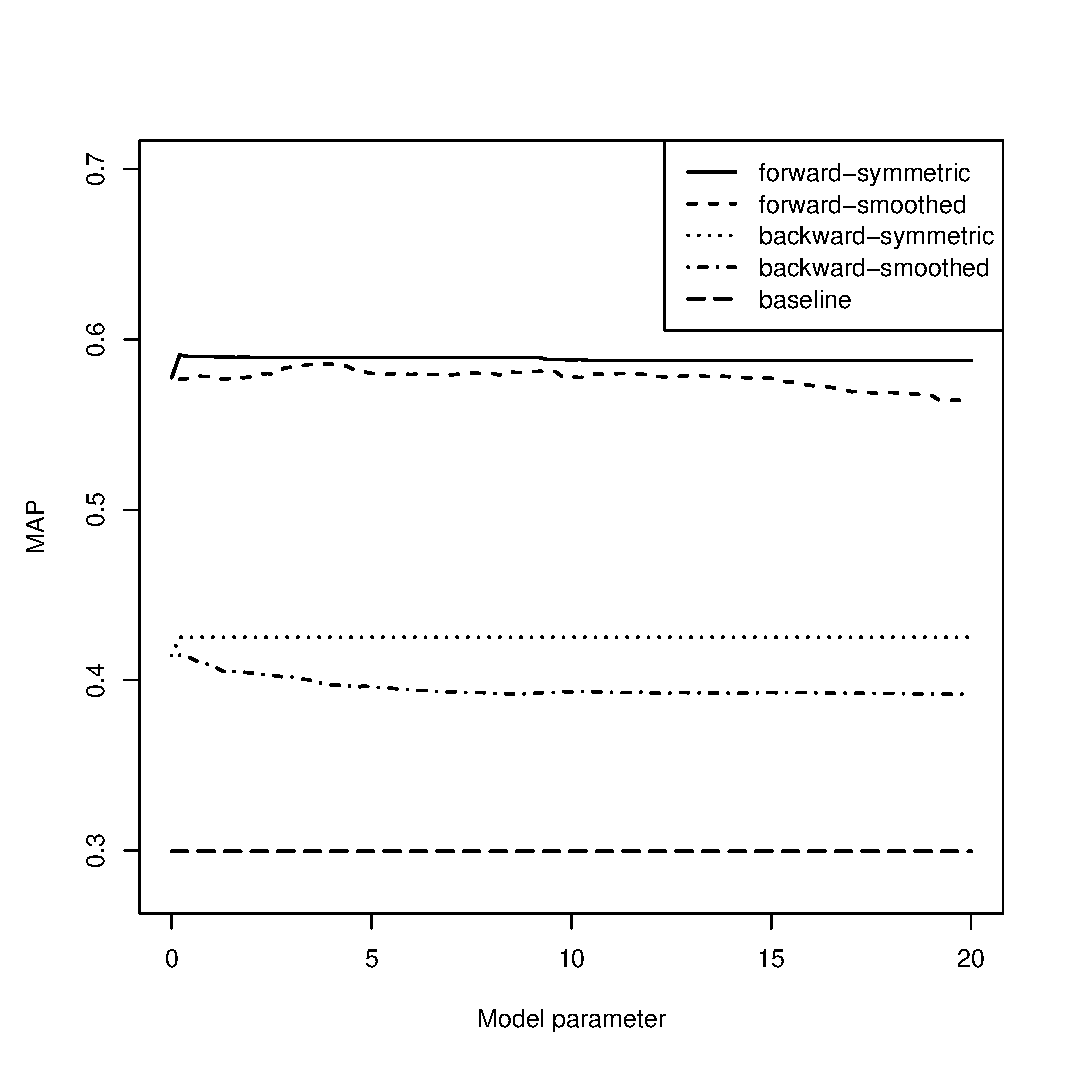
\includegraphics[width=10cm]{performance.eps}
  \caption{The performance results for all the test runs.  The x-axis indicates
  the model parameter: $\beta$ in symmetric model and $\mu$ in smoothed model.
  The y-axis indicates the resulting MAP values.  This figure shows the
  proposed ranking models outperforms the baseline approach across different
  settings of parameters.} \label{f:performance}
\end{figure}

\section{Related Work}\label{s:related-work}

%--------------------------------------------------
% Along with the wide acceptance of faceted search interface in the digital
% library community, an noticable amount of efforts has recently been put on
% usability tests and discovery of more advanced usage.  Previous efforts
% include... \comment{ Related work }
%-------------------------------------------------- 

To the best of our knowledge, this work is among the earliest attempt for retrieving
relevant facets in the digital library community.  What is interesting to note
is that we find similar attempts were already made in the area of expert
finding.  In 2008, Amitay et al. \cite{amitay2008finding} formulated the
problem of expert finding as a two-layered retrieval task and proposed a
solution based on the \emph{inverse entity-frequency}.  Balog et al.
\cite{balog2009language} followed up in the same direction by proposing a
language modeling framework with the similar rationale to extend the use of
language model to the underlying co-occurrence statistics by exploiting
person-term and person-document links.  Our contribution departs from these two
works, not only in the application domain, but in the way document relevance is
incorporated into the model and the support for prior belief.  
 
Our model is inspired by some recent progress on language modeling applications
in information retrieval \cite{lavrenko2001relevance,zaragorza2003bayesian}.
In this aspect, the proposed framework can be seen as a two-stage extension of
the regular language model; however, in considering the integration of prior
knowledge on facet distribution, our model departs from the conventional
language modeling approaches.  

\section{Discussion and Concluding Remarks}\label{s:concluding-remarks}

%--------------------------------------------------
% \comment{ (1 page) The thought flow: \begin{itemize} \item Facet ranking is
% useful in certain applications \begin{itemize} \item Offering an alternative,
% standalone ``relevant facet'' interface for fast navigation.  \item Resource
% selection for generating summary.  \item (Most importantly) Assistance in
% exploratory task. \end{itemize}  \item Our study shows that rank-based model is
% superior to count-based one.  \item We also look into the effect of priors.
% \item Backward model = novelty model?  \item Future direction: benchmark.
% \item Future direction: thorough study on multi-facet dataset. \end{itemize}}
%-------------------------------------------------- 

Our study toward a practical facet ranking algorithm has given rise to a few
interesting questions.  First, all the proposed Bayesian models seem to work
better with smaller priors.  Take the forward models as an example.  According
to the results, the best performance of {\tt forward-symmetric} was achieved
with $\beta = 0.2$ and that of {\tt forward-smoothed} was achieved with $\beta
= 3.6$.  Furthermore, increasing the prior value generally resulted in loss in
retrieval accuracy.  This phenomenon is probably caused by the low average
number of facets in a document.  In our dataset, each document triggers no more
than three facets; larger priors might not work well in this case.  Second, the
result also suggests that the simple symmetric prior being superior to the
smoothed one.  This indicates that, at least in our test collection, the prior
$\Pr(y|C)$ did not make good estimation for $\Pr(y|d)$.  We also found that
models with zero prior (i.e., $\beta = 0$) remains in the top-performer of the
ranking task, suggesting that using the maximum likelihood estimate alone may
already fit the data well.  So far, we do not have a good explanation to this;
a further investigation into the data is needed.

In this work, we proposed a Bayesian language modeling framework for ranking
facets.  We achieved encouraging result on our custom benchmark, improving the
baseline performance by roughly 100\% in MAP.  Moreover, our methods can work
with a language-model-based retrieval engine to achieve high efficiency in
performing the ranking task.  Despite the success in the evaluation results,
there is still room for improving the ranking accuracy.  We see our efforts
here as a starting point toward further exploration on several issues that have
not yet been covered in the study: the use of different distribution families
in the model, a more formal model on the inference for hyperparameters, the
applications on larger datasets, and so on.  These challenges should be the
focus of our future work.

%--------------------------------------------------
% Another interesting aspect that we discovered in the development of testbed
% systems is that users tend to follow top-ranked facets.  According to our
% internal study on the click-through log, the average click-through rank of the
% facets falls in the top 20\% of the presented facets.  This fact also motivates
% our research toward integration of relevance into faceted interface, in which
% users could gain better insight of the content even though they do not explicit
% go through every facet that we discovered.
%-------------------------------------------------- 

%--------------------------------------------------
% Employing a relational database backend is the easiest, while also the most
% practical, approach towards construction of this function.  The document
% contents are usually stored in one table and associated facet records in
% another, and then implement the search function with a plain SQL text match
% against the documents.  The set of facets associated with all the matched
% document and their corresponding counts of occurrences can be pulled out as
% easily with a join or SQL aggregation functions such as {\tt GROUP BY} and {\tt
% COUNT}.  The downside of this approach is we compromise retrieval quality in
% favor of ease of extra efforts because most of the modern relational database
% systems do not really support fuzzy-match in text fields, least to say the
% state-of-the-art document retrieval models.  A proposed workaround for this is
% to host retrieval engine and document representation somewhere else and access
% the RDBMS only for aggregating facet counts.  This could be done fairly easily
% by using the retrieved document identifiers to explicitly form a (probably very
% long) {\tt SELECT} query.  Unfortunately, this solution might not scale well,
% since serving data in an RDBMS way, on the other hand, can obstruct the
% interaction to the retrieval model and degrade the performance.
%-------------------------------------------------- 

\section*{Acknowledgments}

We thank Po-Yu Chen for his support on preparation of the test data.  The
research efforts described in this paper are supported under the National Taiwan
University Digital Archives Project (Project No.  NSC-98-2631-H-002-005), which
is sponsored by National Science Council, Taiwan, 
